\documentclass[letterpaper]{article}
\usepackage{underscore}
\usepackage[left=2.0cm, right=2.0cm, top=2.0cm]{geometry}
\usepackage[utf8]{inputenc}
\usepackage{graphicx}
\usepackage{graphics}
\usepackage[spanish]{babel}
\usepackage{lipsum}
\usepackage{float}
\usepackage{subfigure}
\usepackage{biblatex}
\usepackage{csquotes}
\usepackage{color}

\title{Ev\_2\_Diseño\_de\_un\_modulo\_de\_ancho\_de\_pulso\_(PWM)\_con\_Amp-Op\_y\_transistores}
\author{Joel Alejandro Alcantar Diaz}
\date{October 2019}

\begin{document}

\maketitle
\begin{center}
    
\includegraphics[scale=0.5]{IMG/UPZMGlog.png}\\
    Univerisdad Politecnica de la zona metropolitana de Guadalajara.\\
    4$^to$ A
\end{center}
\newpage
\section{PWM.}
    \begin{large}
        La modulacion de ancho de pulso trata simplemte de controlar el ciclo de trabajo de una señal digital, esto se logra gracias a un oscilador que da señales con una valocidad muy alta a un trancistor dependiendo del voltaje que se quiera en la salida, por ejemplo, si se tiene una señal de corriente directa de 15 volts como es de esperar se tendra en la salida un voltaje de 15 volts si no se switchea, conforme se aumente la velocidad de oscilacion. Digamos que switchea a la mitad de la velocidad de la onda, esto quiere decir que tendremos $\frac{1}{2}$ de la señal original por tanto en cada ciclo habra una mitad en 15 volts y la otra mitad en 0, dando a la salida 7.5 volts, si se mide con un multimetro eso dara, de igual manera si se coloca un capacitor en la salida, siempre y cuando no altenue la señal, tendremos el voltaje de 7.5.\\\\
        Si se mide la onda en un osciloscopio tendremos algo parecido a lo que se muestra en la figura 1.
        \begin{figure}[htbp]
            \centering
            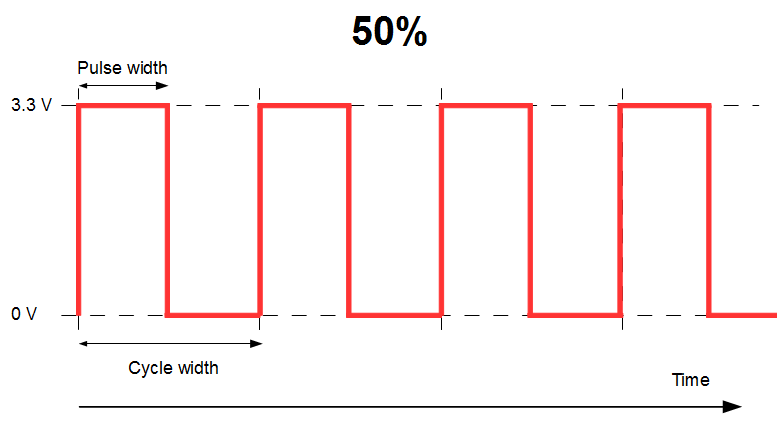
\includegraphics[scale=0.5]{IMG/50.png}
            \caption{Modulacion al 50\%}
            \label{fig:50per}
        \end{figure}
        En la figura 1 se puede apreciar como el tamaño del trabajo es de la mitad del ciclo dando como resultado la mitad del voltaje suministrado a la entrada.
        Este tipo de regulador de voltaje, por asi decirlo, es mas eficiete que el solo poner una resitencia ya que no tiene perdidas disipadas en calor colo lo tendria una resistencia.\\\\
        Para calcular el porcentaje de trabajo del ciclo se aplica la siguiente formula:\\
        \begin{center}
            $D=\frac{T_{Trabajo}}{T_{Ciclo}}$
        \end{center}
    \end{large}
    \section{Diseño de controlador de ancho de pulso (PWM)}
    En este circuito se propone una configuracion para el control de pulso, como carga se utiliza un motor.
    \newpage
    \begin{figure}
        \centering
        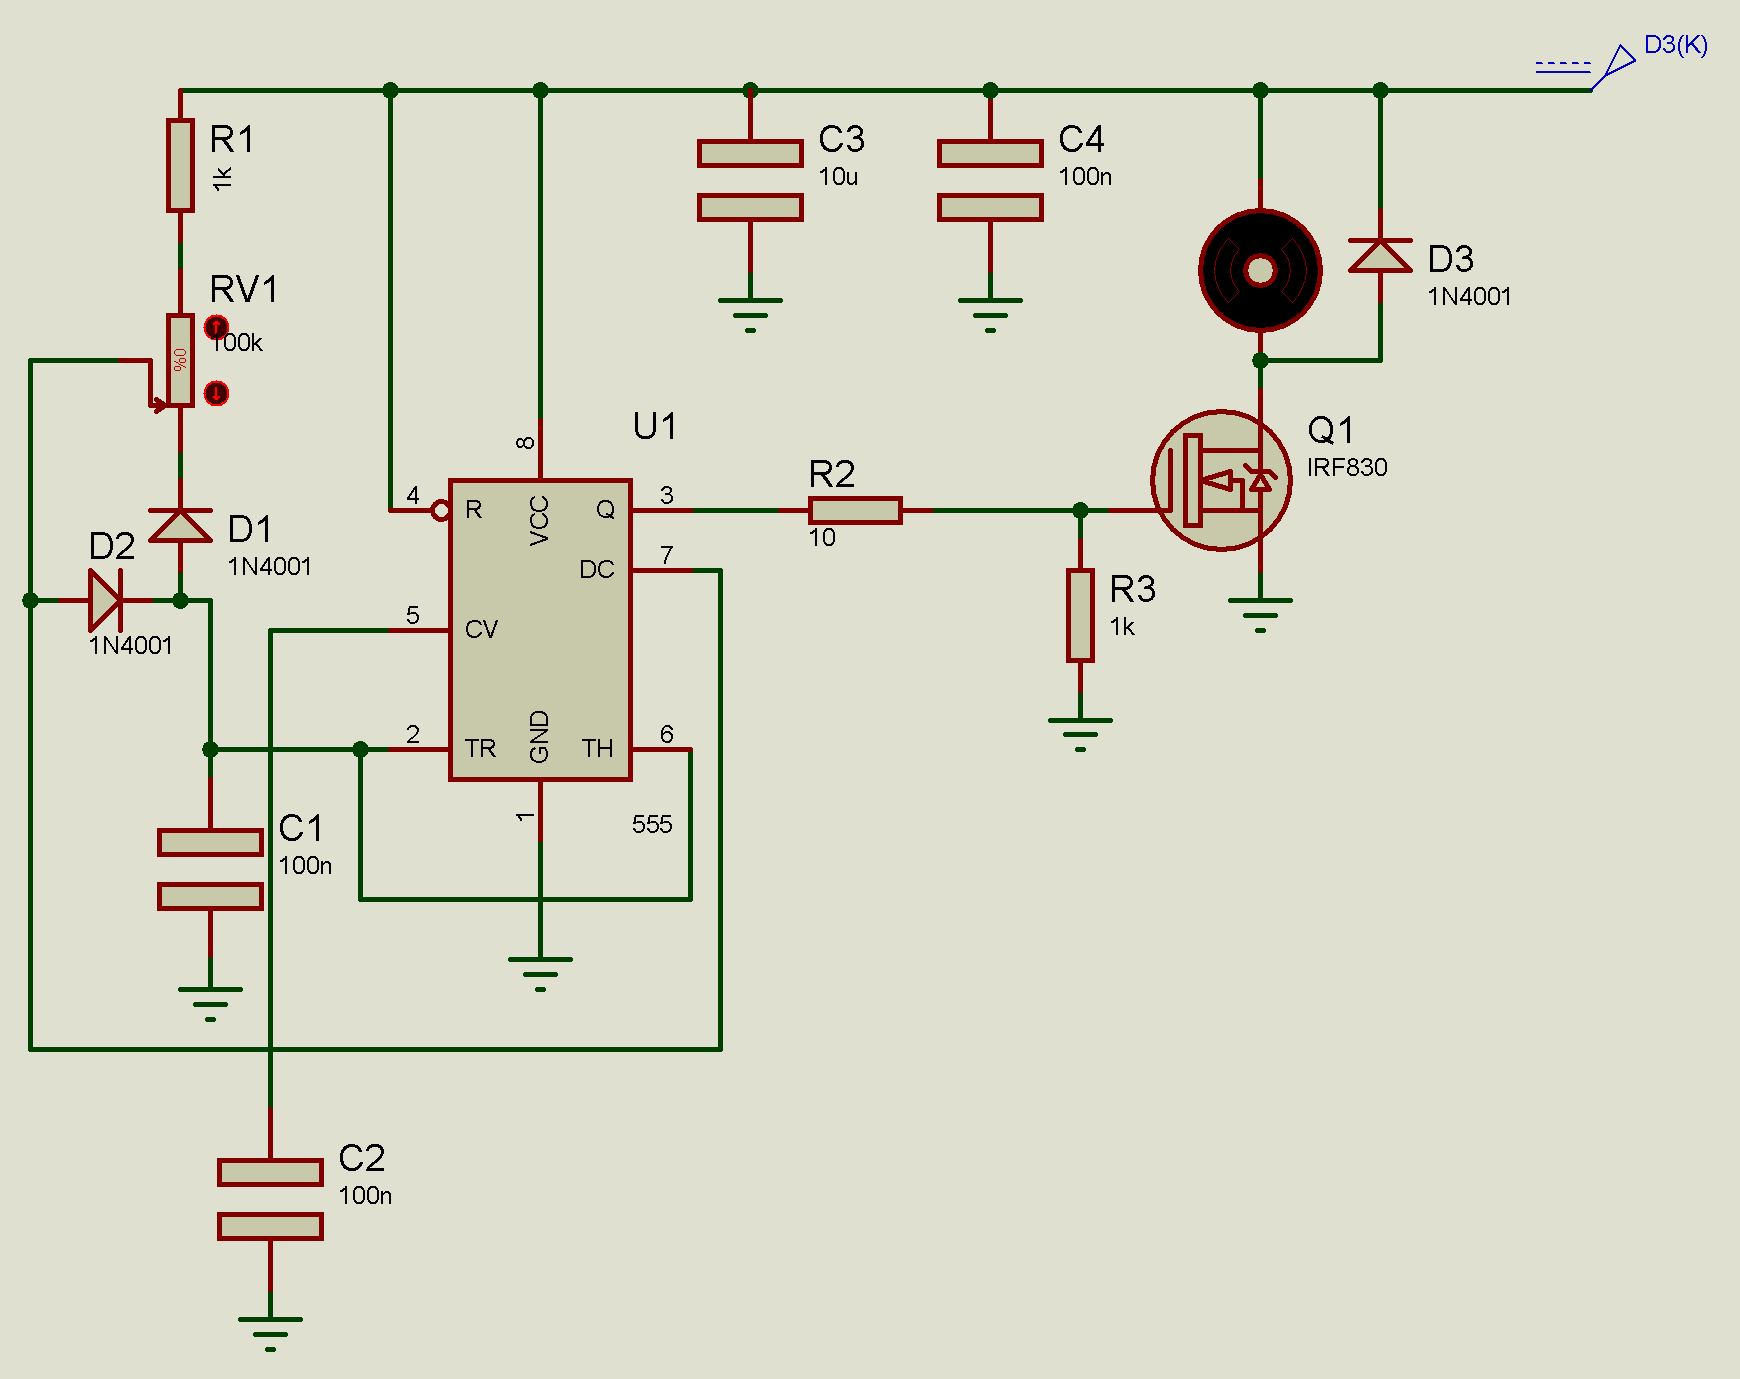
\includegraphics[scale=0.3]{IMG/PMW.png}
        \caption{Diagrama de un controlador de pulso.}
        \label{fig:diag}
    \end{figure}

\end{document}
